%%%%%%%%%%%%%%%%%%%%%%%%%%%%%%%%%%%%%%%%%%%%%%%%%%%%%%%%%%%%
%%  This Beamer template was created by Cameron Bracken.
%%  Anyone can freely use or modify it for any purpose
%%  without attribution.
%%
%%  Last Modified: January 9, 2009
%%

\documentclass[xcolor=x11names,compress]{beamer}

%% General document %%%%%%%%%%%%%%%%%%%%%%%%%%%%%%%%%%
\usepackage{graphicx}
\usepackage{tikz}
\usetikzlibrary{decorations.fractals}
%%%%%%%%%%%%%%%%%%%%%%%%%%%%%%%%%%%%%%%%%%%%%%%%%%%%%%


%% Beamer Layout %%%%%%%%%%%%%%%%%%%%%%%%%%%%%%%%%%
\useoutertheme[subsection=false,shadow]{miniframes}
\useinnertheme{default}
\usefonttheme{serif}
\usepackage{palatino}

\setbeamerfont{title like}{shape=\scshape}
\setbeamerfont{frametitle}{shape=\scshape}

\setbeamercolor*{lower separation line head}{bg=DeepSkyBlue4} 
\setbeamercolor*{normal text}{fg=black,bg=white} 
\setbeamercolor*{alerted text}{fg=red} 
\setbeamercolor*{example text}{fg=black} 
\setbeamercolor*{structure}{fg=black} 
 
\setbeamercolor*{palette tertiary}{fg=black,bg=black!10} 
\setbeamercolor*{palette quaternary}{fg=black,bg=black!10} 

\renewcommand{\(}{\begin{columns}}
\renewcommand{\)}{\end{columns}}
\newcommand{\<}[1]{\begin{column}{#1}}
\renewcommand{\>}{\end{column}}
%%%%%%%%%%%%%%%%%%%%%%%%%%%%%%%%%%%%%%%%%%%%%%%%%%




\begin{document}


%%%%%%%%%%%%%%%%%%%%%%%%%%%%%%%%%%%%%%%%%%%%%%%%%%%%%%
%%%%%%%%%%%%%%%%%%%%%%%%%%%%%%%%%%%%%%%%%%%%%%%%%%%%%%
\section{\scshape Introduction}
\begin{frame}
\title{Article Review and Project Overview}
%\subtitle{SUBTITLE}
\author{
	Cameron Bracken\\
	CVEN 6833\\
}
\date{
	\begin{tikzpicture}[decoration=Koch curve type 2] 
		\draw[DeepSkyBlue4] decorate{ decorate{ decorate{ (0,0) -- (3,0) }}}; 
	\end{tikzpicture}  
	\\
	\vspace{1cm}
	{December 9, 2009}
}
\titlepage
\end{frame}

%%%%%%%%%%%%%%%%%%%%%%%%%%%%%%%%%%%%%%%%%%%%%%%%%%%%%%
%%%%%%%%%%%%%%%%%%%%%%%%%%%%%%%%%%%%%%%%%%%%%%%%%%%%%%
\begin{frame}{Introduction}
\begin{itemize}
\item {\bf Review of article}:

\begin{itemize}
\item Lall, U., Y.I. Moon, H.H. Kwon, and K. Bosworth (2006), Locally weighted polynomial regression: Parameter choice and application to forecasts of the Great Salt Lake, Water Resour. Res., 42, W05422, doi:10.1029/2004WR003782.
\end{itemize}

\item \bf Overview of project
\end{itemize}
\end{frame}

%%%%%%%%%%%%%%%%%%%%%%%%%%%%%%%%%%%%%%%%%%%%%%%%%%%%%%
%%%%%%%%%%%%%%%%%%%%%%%%%%%%%%%%%%%%%%%%%%%%%%%%%%%%%%
\section{Article Review}
\subsection{Overview}
\begin{frame}{Lall et al. (2006) - Overview}

\begin{itemize}
\item General (qualitative) discussion of locally weighted polynomial (LWP) regression
\pause
\item Non-Rigorous development of LWP model, discussing parameter choice ($k$, $p$)
\pause
\item Definition of new local perdictive error estimator ($LGCVLEV$)
\pause
\item Application to forecast of Great Salt Lake Volume
\end{itemize}

\end{frame}

%%%%%%%%%%%%%%%%%%%%%%%%%%%%%%%%%%%%%%%%%%%%%%%%%%%%%%
%%%%%%%%%%%%%%%%%%%%%%%%%%%%%%%%%%%%%%%%%%%%%%%%%%%%%%
\subsection{Background}
\begin{frame}{Background}
\begin{itemize}
\item Directed discussion of locally weighted polynimials from ``first principals''
\pause
\item Focus on pacticality
	\begin{itemize}
	\item Scaling of data
	\item Limits on parameter choices (eg. $k>2n_p$ )
	\item Weight function 
	\end{itemize}
\pause
\item Distinction between ``smoothing parameters'' ($k$ and $p$) and ``Structural parameters'' ($\mathbf{\beta}_l$, $\hat{f}(\mathbf{x}_l) = \mathbf{z}_l\beta_l$)
\pause
\item Presentation of useful statistical quantities ($s^2_{e_l}$)
\end{itemize}
\end{frame}

%%%%%%%%%%%%%%%%%%%%%%%%%%%%%%%%%%%%%%%%%%%%%%%%%%%%%%
%%%%%%%%%%%%%%%%%%%%%%%%%%%%%%%%%%%%%%%%%%%%%%%%%%%%%%
\subsection{GCV and LGCV}
\begin{frame}{GGCV and LGCV}
$$GGCV(\hat{f})=\frac{\mathbf{e}^T\mathbf{e}/n}{\left(1-tr(H)/n\right)^2}$$
$$LGCV_l(\hat{f})=\frac{\mathbf{e}^T_lW_l\mathbf{e}^T_l/n}{\left(1-n_p'/k\right)^2}$$

\begin{itemize}
	\item Useful measures of predictive error
	\item Related to OCV and AIC
	\item Assume ``regular or well behaved sampling of the data''
	\item Poor performance with local data clustering
\end{itemize}
\end{frame}

%%%%%%%%%%%%%%%%%%%%%%%%%%%%%%%%%%%%%%%%%%%%%%%%%%%%%%
%%%%%%%%%%%%%%%%%%%%%%%%%%%%%%%%%%%%%%%%%%%%%%%%%%%%%%
\subsection{GCV and LGCV}
\begin{frame}{GGCV and LGCV}
$$LGCVLEV(z_n)=LGCV_lh_l$$
$$h_l=\mathbf{z}(Z_l^TW_lZ_l)^{-1}\mathbf{z}_l^T/k$$

\begin{itemize}
	\item Uses leverage, $h_l$, of the point of estimation on the data set
	\item Leverage increases further away from data point
	\item Leverage is a ``penalty to account for the degree of extrapolation''
\end{itemize}
\end{frame}

%%%%%%%%%%%%%%%%%%%%%%%%%%%%%%%%%%%%%%%%%%%%%%%%%%%%%%
%%%%%%%%%%%%%%%%%%%%%%%%%%%%%%%%%%%%%%%%%%%%%%%%%%%%%%
\subsection{GCV and LGCV}
\begin{frame}{LLGCVLEV}
\centering
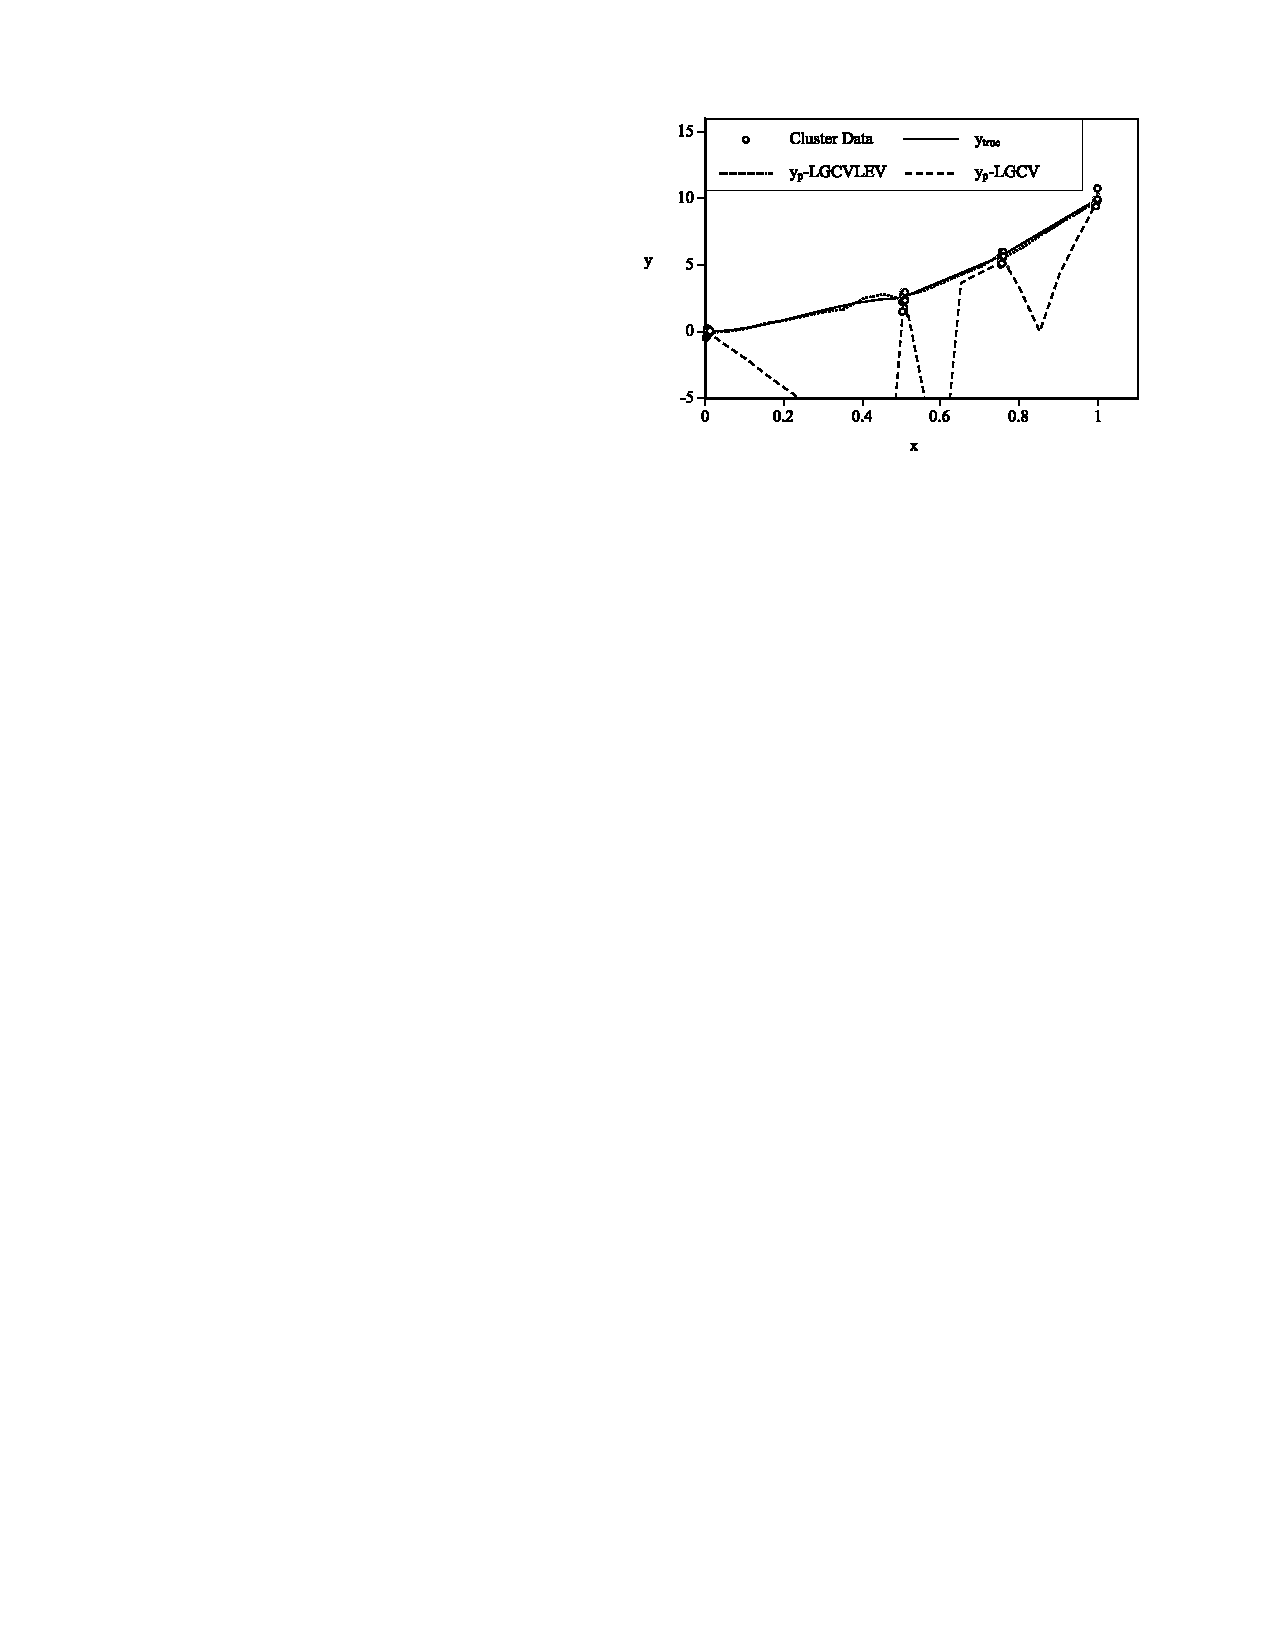
\includegraphics[width=.7\textwidth]{LGCVLEV.pdf}
\end{frame}


%%%%%%%%%%%%%%%%%%%%%%%%%%%%%%%%%%%%%%%%%%%%%%%%%%%%%%
%%%%%%%%%%%%%%%%%%%%%%%%%%%%%%%%%%%%%%%%%%%%%%%%%%%%%%
\subsection{Methodology}
\begin{frame}{Application to GSL forecast}
Given timesries $G_t,$, $t=1,...,nt$, the $m$ step ahead forecast model is
$$G_{t+m}=f_m({V_t})+e_t$$
$$V_t=(G_t, G_{t-1}, ..., G_{t-(m_1)\tau})$$
\begin{itemize}
	\item Iterated forecast
	\item Reconstruct $f_m$ at each step $m$ based on updated $V_t$ using LWP model of embedded timeseries
\end{itemize}
\end{frame}

\begin{frame}{Application to GSL forecast}
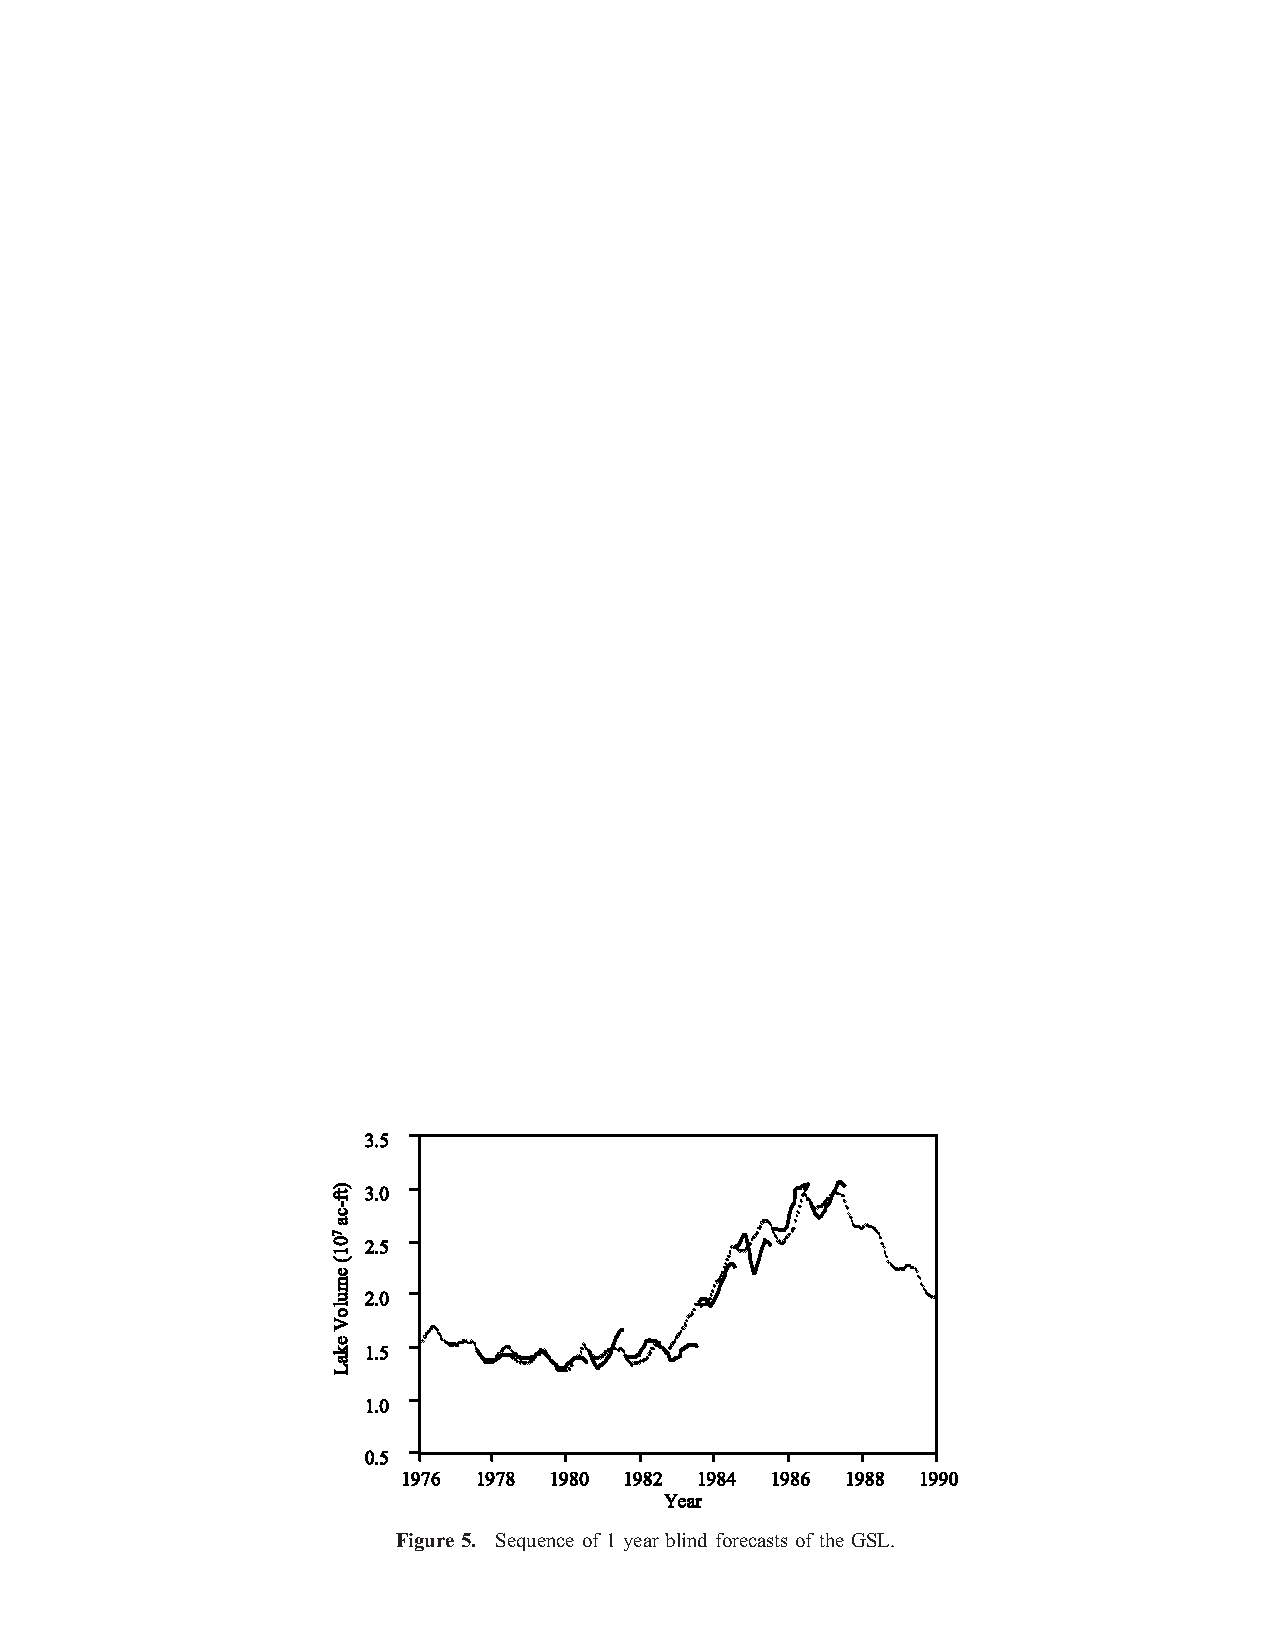
\includegraphics[width=.8\textwidth]{fc.pdf}
\end{frame}

%%%%%%%%%%%%%%%%%%%%%%%%%%%%%%%%%%%%%%%%%%%%%%%%%%%%%%
%%%%%%%%%%%%%%%%%%%%%%%%%%%%%%%%%%%%%%%%%%%%%%%%%%%%%%
\subsection{Comments}
\begin{frame}{Comments}

\begin{itemize}
\item Major contribution was $LGCVLEV$
\item Compact discussion and clear algorithmic reprepresentation of LWP
	\begin{itemize}
		\item Focus on choice of ``smoothing parameters'' which maximize predicability
	\end{itemize}
\end{itemize}

\end{frame}


%%%%%%%%%%%%%%%%%%%%%%%%%%%%%%%%%%%%%%%%%%%%%%%%%%%%%%
%%%%%%%%%%%%%%%%%%%%%%%%%%%%%%%%%%%%%%%%%%%%%%%%%%%%%%
\section{Project Overview}
\subsection{Project Overview - My Research}
\begin{frame}{Project Overview - My Research}
\framesubtitle{Probabilistic Midterm Model}
\pause
\begin{itemize}
\item Midterm operational forecast model for the CRB
\item Augment the 24 month study
\item New features
	\begin{itemize}
	\item Multiple traces
	\item Demands 
	\item Operational rules
	\item Real time data inputs
	\item Second year forecasts
	\end{itemize}
\end{itemize}
\end{frame}

%%%%%%%%%%%%%%%%%%%%%%%%%%%%%%%%%%%%%%%%%%%%%%%%%%%%%%
%%%%%%%%%%%%%%%%%%%%%%%%%%%%%%%%%%%%%%%%%%%%%%%%%%%%%%
\subsection{Methodology}
\begin{frame}{Second Year Forecast Considerations}
\begin{itemize}
\item Current models use climatology
	\begin{itemize}
		\item Especially bad for successive dry or wet periods
		\item No user confidence in current forecast beyond 1 year
	\end{itemize}
\item Little or no skill from climate or snow, need a different approach
\end{itemize}
\end{frame}

%%%%%%%%%%%%%%%%%%%%%%%%%%%%%%%%%%%%%%%%%%%%%%%%%%%%%%
%%%%%%%%%%%%%%%%%%%%%%%%%%%%%%%%%%%%%%%%%%%%%%%%%%%%%%
\subsection{Methodology}
\begin{frame}{Approach}
\textbf{Forecast 2nd year total volume}:
	\begin{itemize}
	\item KNN bootstrap
	\pause
	\item Markov Approach (2-5 years) using paleoclimate state information
	\begin{itemize}
		\item Basic window resampling
	\end{itemize}
	\item More persistant predictors such as ENSO/PDO
	\end{itemize}
\end{frame}


%%%%%%%%%%%%%%%%%%%%%%%%%%%%%%%%%%%%%%%%%%%%%%%%%%%%%%
%%%%%%%%%%%%%%%%%%%%%%%%%%%%%%%%%%%%%%%%%%%%%%%%%%%%%%
\subsection{Application}
\begin{frame}{Application}
\begin{itemize}
\item Lees Ferry (long period of record)
\pause
\item Measure usefulness in terms of an operational variable
	\begin{itemize}
		\item Power
		\item Reservoir drawdown leading to triggers
	\end{itemize}
\pause
\item Hope to show early predictability of 2002 event as a proof of concept
\end{itemize}
\end{frame}


\end{document}